\documentclass[12pt,oneside,a4paper,parskip]{scrbook}
\usepackage[utf8]{inputenc}
\usepackage{csquotes}
\usepackage[ngerman]{babel}
\usepackage{floatflt}
\usepackage{subfigure}
\usepackage[pdftex]{graphicx}
\usepackage[hidelinks]{hyperref}
\usepackage{color}
\usepackage{amssymb}
\usepackage{textcomp}
\usepackage{nicefrac}
\usepackage{scrhack}
\usepackage{pdfpages}
\usepackage{float}
\usepackage{pdflscape}
\usepackage{subfigure}
\usepackage{pdfpages}
\usepackage[verbose]{placeins}
%\usepackage[nouppercase,headsepline,plainfootsepline]{scrpage2}
\usepackage{listings}
\usepackage{xcolor}
\usepackage{color}
\usepackage{caption}
\usepackage{subfigure}
\usepackage{epstopdf}
\usepackage{longtable}
\usepackage{setspace}
\usepackage{booktabs}
\usepackage[style=numeric,backend=biber, uniquelist=false]{biblatex}
\bibliography{literatur}
\addbibresource{literatur.bib}


%%%%%%%%%%%%%%%%%%%
%% definitions
%%%%%%%%%%%%%%%%%%%
\def\BaAuthor{David Mödl\, Sebastian Lober}
\def\BaAuthorStudyProgram{Informatik} %% Wirtschaftsinformatik, E-Commerce, Informationssysteme
\def\BaType{Seminararbeit} %% Masterarbeit
\def\BaTitle{Bias of Neural Networks - Security implications}
\def\BaSupervisorOne{Prof.\ Dr.\ A B}
\def\BaSupervisorTwo{Prof.\ Dr.\ C D}
\def\BaDeadline{\today}

\ifdefined\iswithfullname
  \def\ShowBaAuthor{\BaAuthor}
\else
  \def\ShowBaAuthor{N.~N.}
\fi

\hypersetup{
pdfauthor={\ShowBaAuthor},
pdftitle={\BaTitle},
pdfsubject={Subject},
pdfkeywords={Keywords}
}

%%%%%%%%%%%%%%%%%%%
%% configs to include
%%%%%%%%%%%%%%%%%%%
\colorlet{punct}{red!60!black}
\definecolor{background}{HTML}{EEEEEE}
\definecolor{delim}{RGB}{20,105,176}
\colorlet{numb}{magenta!60!black}

\definecolor{gray}{rgb}{0.4,0.4,0.4}
\definecolor{darkblue}{rgb}{0.0,0.0,0.6}
\definecolor{cyan}{rgb}{0.0,0.6,0.6}

\definecolor{pblue}{rgb}{0.13,0.13,1}
\definecolor{pgreen}{rgb}{0,0.5,0}
\definecolor{pred}{rgb}{0.9,0,0}
\definecolor{pgrey}{rgb}{0.46,0.45,0.48}

\lstset{
  basicstyle=\ttfamily,
  columns=fullflexible,
  showstringspaces=false,
  commentstyle=\color{gray}\upshape
  linewidth=\textwidth
}

\lstdefinelanguage{json}{
    basicstyle=\normalfont\ttfamily,
    numbers=left,
    numberstyle=\scriptsize,
    stepnumber=1,
    numbersep=8pt,
    showstringspaces=false,
    breaklines=true,
    backgroundcolor=\color{background},
    literate=
     *{0}{{{\color{numb}0}}}{1}
      {1}{{{\color{numb}1}}}{1}
      {2}{{{\color{numb}2}}}{1}
      {3}{{{\color{numb}3}}}{1}
      {4}{{{\color{numb}4}}}{1}
      {5}{{{\color{numb}5}}}{1}
      {6}{{{\color{numb}6}}}{1}
      {7}{{{\color{numb}7}}}{1}
      {8}{{{\color{numb}8}}}{1}
      {9}{{{\color{numb}9}}}{1}
      {:}{{{\color{punct}{:}}}}{1}
      {,}{{{\color{punct}{,}}}}{1}
      {\{}{{{\color{delim}{\{}}}}{1}
      {\}}{{{\color{delim}{\}}}}}{1}
      {[}{{{\color{delim}{[}}}}{1}
      {]}{{{\color{delim}{]}}}}{1},
}

\lstset{language=xml,
  morestring=[b]",
  morestring=[s]{>}{<},
  morecomment=[s]{<?}{?>},
  stringstyle=\color{black},
  numbers=left,
  numberstyle=\scriptsize,
  stepnumber=1,
  numbersep=8pt,
  identifierstyle=\color{darkblue},
  keywordstyle=\color{cyan},
  backgroundcolor=\color{background},
  morekeywords={xmlns,version,type}% list your attributes here
}

\lstset{language=Java,
  showspaces=false,
  showtabs=false,
  tabsize=4,
  breaklines=true,
  keepspaces=true,
  numbers=left,
  numberstyle=\scriptsize,
  stepnumber=1,
  numbersep=8pt,
  showstringspaces=false,
  breakatwhitespace=true,
  commentstyle=\color{pgreen},
  keywordstyle=\color{pblue},
  stringstyle=\color{pred},
  basicstyle=\ttfamily,
  backgroundcolor=\color{background},
%  moredelim=[il][\textcolor{pgrey}]{$$},
%  moredelim=[is][\textcolor{pgrey}]{\%\%}{\%\%}
}

\newcommand*{\forcetwosidetitle}[1][1]{%
 \begingroup
   \cleardoubleoddpage
   \KOMAoptions{titlepage=true}% useful e.g. for scrartcl
   \csname @twosidetrue\endcsname
   \maketitle[{#1}]
 \endgroup
}


\begin{document}


%%%%%%%%%%%%%%%%%%%
%% Titelseite
%%%%%%%%%%%%%%%%%%%


\frontmatter
\titlehead{%  {\centering Seitenkopf}
  {Hochschule für angewandte Wissenschaften Würzburg-Schweinfurt\\
   Fakultät Informatik und Wirtschaftsinformatik}}
\subject{\BaType}
\title{\BaTitle\\[15mm]}
%\subtitle{\normalsize{vorgelegt an der Hochschule f\"{u}r angewandte Wissenschaften W\"{u}rzburg-Schweinfurt in der Fakult\"{a}t Informatik und Wirtschaftsinformatik zum Abschluss eines Studiums im Studiengang \BaAuthorStudyProgram}}
\author{David Mödl \& Sebastian Lober}
%\date{\normalsize{Eingereicht am: \BaDeadline}}
%\publishers{
%  \normalsize{Erstpr\"{u}fer: \BaSupervisorOne}\\
%  \normalsize{Zweitpr\"{u}fer: \BaSupervisorTwo}\\
%}
\forcetwosidetitle


%%%%%%%%%%%%%%%%%%%
%% abstract
%%%%%%%%%%%%%%%%%%%

\section*{Zusammenfassung}

TODO

\section*{Abstract}

TODO



%%%%%%%%%%%%%%%%%%%
%% Inhaltsverzeichnis
%%%%%%%%%%%%%%%%%%%
\tableofcontents



%%%%%%%%%%%%%%%%%%%
%% Main part of the thesis
%%%%%%%%%%%%%%%%%%%
\mainmatter

\chapter{Einführung}
\label{chapter:intro}
Künstliche Intelligenz(KI) oder auch artifizielle Intelligenz(AI) tritt in großen Teilen unserer Gesellschaft auf. Von Kaufvorschlägen in Amazon, über Chat-Bots bis hin zu autonom fahrenden Autos spielt die KI eine große Rolle. Die künstliche Intelligenz beschäftigt sich mit Methoden, die es einem Computer ermöglichen, Aufgaben zu lösen, die, wenn sie vom Menschen gelöst werden Intelligenz erfordern \cite{kiDefinition}.
\\\\
Um dieses Wissen aufzubauen, wird z.B. durch maschinelles Lernen ein System mit Beispieldaten trainiert. 
Diese Trainingsdaten bestehen aus mehreren Datensätzen, welche eine Gruppe von inhaltlich zusammenhängenden Datenfeldern sind, z.B. Artikelnummer und Artikelname.
Mit Hilfe von Algorithmen wird aus diesen Beispielen ein statisches Modell aufgebaut. Dass heißt, es werden nicht einfach die Beispiele auswendig gelernt, sondern Muster und Gesetzmäßigkeiten in den Lerndaten erkannt. So kann das System unbekannte Daten beurteilen und Ergebnisse vorhersagen.
\\\\
Dabei hängt die Genauigkeit und Präzision dieser Beurteilung von dem Trainingsdaten ab. Je breiter die Daten zum Lernen aufgestellt sind, also je mehr Fälle durch diese Daten abgedeckt werden, umso genauer wird der Algorithmus die unbekannten Daten beurteilen können. Ein weiterer Vorteil dadurch ist, dass die Chance erhöht wird, Vorurteile, welche in den Datensätzen vorkommen können, zu eliminieren.\\
Diese Vorurteile können ansonsten zu Fehlverhalten und Sicherheitsprobleme der KI führen. In dieser Arbeit möchten wir auf diese Fehlverhalten eingehen, welche Sicherheitsprobleme dadurch auftreten können und erläutern wie diese vermieden werden können.


\chapter{Grundlagen KI}

\section{Künstliche Intelligenz?}
KI steht kurz für künstliche Intelligenz. Der Begriff KI ist jedoch irreführend. Eine 'KI' ist ein Programm, das versucht biologisches intelligentes Verhalten nachzuahmen. Die Begrifflichkeit Intelligenz in Verbindung mit Computern ist sehr umstritten, dennoch wird im Allgemeinen als auch in der Forschung das Wort 'Intelligenz' verwendet. \\
Aus diesem Grund und an Mangel an qualitativ hochwertigen Alternativen wird auch im Folgenden der Wortlaut KI verwendet, wohl wissend, dass die Bezeichnung nicht 100 Prozent korrekt ist.
\section{Machine Learning}
% "Maschinelles Lernen ist ein Oberbegriff für die „künstliche“ Generierung von Wissen aus Erfahrung" Quelle Wiki 
% -> Dementsprechend ist künstliche Intelligenz ein Teilgebiet von Machine Learning
% "Zu unterscheiden ist der Begriff [Machine Learning] zudem von dem Begriff „Deep Learning“, welches nur eine mögliche Lernvariante mittels künstlicher neuronaler Netze darstellt." Quelle Wiki
% https://de.wikipedia.org/wiki/Maschinelles_Lernen
Machine Learning (ML) ist ein Teilgebiet der künstlichen Intelligenz. Wie in \ref{chapter:intro} beschrieben, werden Systeme mit Hilfe von Machine Learning trainiert, indem durch die Trainingsdaten, Muster und Gesetzmäßigkeiten erkannt werden. Die aus den Daten gewonnenen Erkenntnisse lassen sich verallgemeinern und für neue Problemlösungen oder für die Analyse von bisher unbekannten Daten verwenden.\\
Das Ergebnis aus der Analyse von unbekannten Daten, soll wiederum in den Lernprozess für weitere neue Daten integriert werden. Das Hauptziel ist, dass die Maschine automatisch lernt ohne vom Menschen Hilfe oder Anweisungen zu bekommen und daraufhin die Aktionen von alleine anpasst\cite{EliminateHumanBias}.
\\\\
Damit das System eigenständig lernen und Lösungen finden kann, ist ein vorheriges Handeln von Menschen notwendig. Beispielsweise müssen die Systeme zunächst mit den für das Lernen relevanten Daten und Algorithmen versorgt werden.
Je mehr Trainingsdaten in den Maschine geladen werden, desto besser wird die Performance des Algorithmus.\\
% Tipp: Nächsten Absatz umformulieren
Zudem sind Regeln für die Analyse des Datenbestandes und das Erkennen der Muster aufzustellen. Sind passende Daten vorhanden und Regeln definiert, können Systeme mit maschinellem Lernen unter anderem folgendes:

\begin{enumerate}
	\item Relevante Daten finden, extrahieren und zusammenfassen,
	\item Vorhersagen auf Basis der analysierten Daten treffen,
	\item Wahrscheinlichkeiten für bestimmte Ereignisse berechnen,
	\item sich an Entwicklungen eigenständig anpassen und
	\item Prozesse auf Basis erkannter Muster optimieren.
\end{enumerate}


\section{Was sind neuronale Netzwerke?}
Bilderkennung ist beispielsweise ein Gebiet, bei den neuronale Netzwerke heutzutage angewandt werden. Gibt man bei einer Suchmaschine ein beliebiges Wort ein, werden direkt hunderte Bilder diesbezüglich angezeigt. Auch ist es möglich Bilder hochzuladen. Ein neuronales Netzwerk interpretiert die hochgeladene Datei und ähnliche bis gleiche Bilder werden angezeigt. 
\\\\
Hochauflösende Bilder bestehen aus mehreren Millionen Pixel mit Position und meist RGB-Werten für die Farbe des Punktes. 
% Bearbeiten
Nur durch Verbindung der richtigen einzelnen Punkte könnte man Konturen erkennen. 
%
Diese müssen dann der richtigen Kategorie zugeordnet werden, um sie bei einem Suchwort wie 'Haus' anzuzeigen. Doch wie kann ein Computer aus dieser riesigen Menge an einzelnen Pixeln Bilder richtig kategorisieren?
\\\\
Wir Menschen nehmen Bilder mit der Netzhaut des Auges als visuelle Reize auf und senden sie an unser Gehirn. Dieses verarbeitet die Informationen durch einen Teil der etwa 100 Milliarden Neuronen. Jedes Neuron hat 1 bis 200.000 Synapsen, also Verbindungen zu anderen Neuronen. Durch dieses Geflecht an Neuronen werden die Informationen als elektrische Reize durchgeschleust. %durchgeschleust evtl ersetzen
\\\\
Diesen Prozess der Informationsverarbeitung wird in der Informatik mit künstlichen Neuronen und Synapsen versucht nachzuahmen. 
\section{Wie funktionieren künstliche neuronale Netzwerke?}
Ein künstliches neuronales Netzwerk besteht aus künstlichen Neuronen.\\

\begin{figure}[ht]
	\begin{center}
		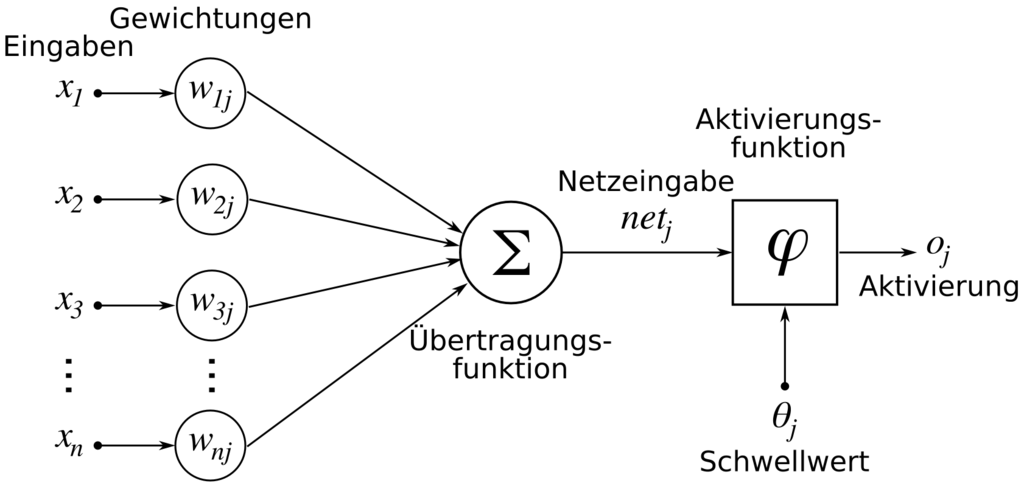
\includegraphics[width=12cm]{Bilder/ArtificialNeuronModel_deutsch.png}
		\caption{Künstliches Neuron}
		\label{fig:wikiNeuron}
	\end{center}
\end{figure}
% https://de.wikipedia.org/wiki/K%C3%BCnstliches_Neuron#/media/Datei:ArtificialNeuronModel_deutsch.png

Ein Neuron besitzt mehrere Eingangskanäle 
% Eingaben
und einen Ausgangskanal, das sind die Verbindungen bzw. Synapsen. Wenn das Neuron über die Eingangskanäle genügend stimuliert wird,
% Aktivierungsfunktion
 feuert das Neuron ein Signal 
% Aktivierung
an den Ausgangskanal. Im Gehirn sind einige Eingangskanäle wichtiger als andere, in der Informatik wird dies mit Gewichtungen gelöst. 
\\\\
Auch ist jedes Neuron mehr oder weniger sensibel. Somit muss durch die gewichteten Eingangskanäle 
% Übertragungsfunktion
ein gewisser Schwellwert summiert anliegen.
% Netzeingabe
Wenn dieser Schwellwert 
% Aktivierungsfunktion
erreicht wird, feuert das Neuron.
% Aktivierung
Der Ausgangskanal eines Neuron ist gleichzeitig ein Eingangskanal eines oder mehreren anderen Neuronen.
\\\\
Dadurch dass ein Neuron mehrere Eingangskanäle besitzt, werden viele Eingangsinformationen auf eine Ergebnis reduziert. Durch mehrere Schichten und vielen Neuronen pro Schicht kann so eine große Menge an Daten schnell reduziert werden. 
\\\\
Jedoch muss ein künstliches neurales Netzwerk erst trainiert werden. Trainieren bedeutet hier das Einstellen der Gewichtungen von Verbindungen und Schwellwerte der Neuronen für eine spezielle Aufgabe. Diesen Prozess nennt man Deep Learning eine Form von Machine Learning.

\section{Deep Learning}

%indem durch die Trainingsdaten, Muster und Gesetzmäßigkeiten erkannt werden. Die aus den Daten gewonnenen Erkenntnisse lassen sich verallgemeinern und für neue Problemlösungen oder für die Analyse von bisher unbekannten Daten verwenden.\\
% Das Ergebnis aus der Analyse von unbekannten Daten, soll wiederum in den Lernprozess für weitere neue Daten integriert werden. Das Hauptziel ist, dass die Maschine automatisch lernt ohne vom Menschen Hilfe oder Anweisungen zu bekommen und daraufhin die Aktionen von alleine anpasst\cite{EliminateHumanBias}.

Beim Deep Learning werden die zahlreichen Zwischenschichten, eingeschlossen von Eingabe- und Ausgabe-Schicht, trainiert. Hierbei wird eine umfangreiche und komplexe Struktur der Neuronen-Verbindungen zwischen den Schichten aufgebaut. Wie das Programm endgültig die Aufgabe lösen soll, wird hierbei nicht vorgegeben, sondern wird bei diesem Prozess autonom ermittelt.
\begin{figure}[h]
	\begin{center}
		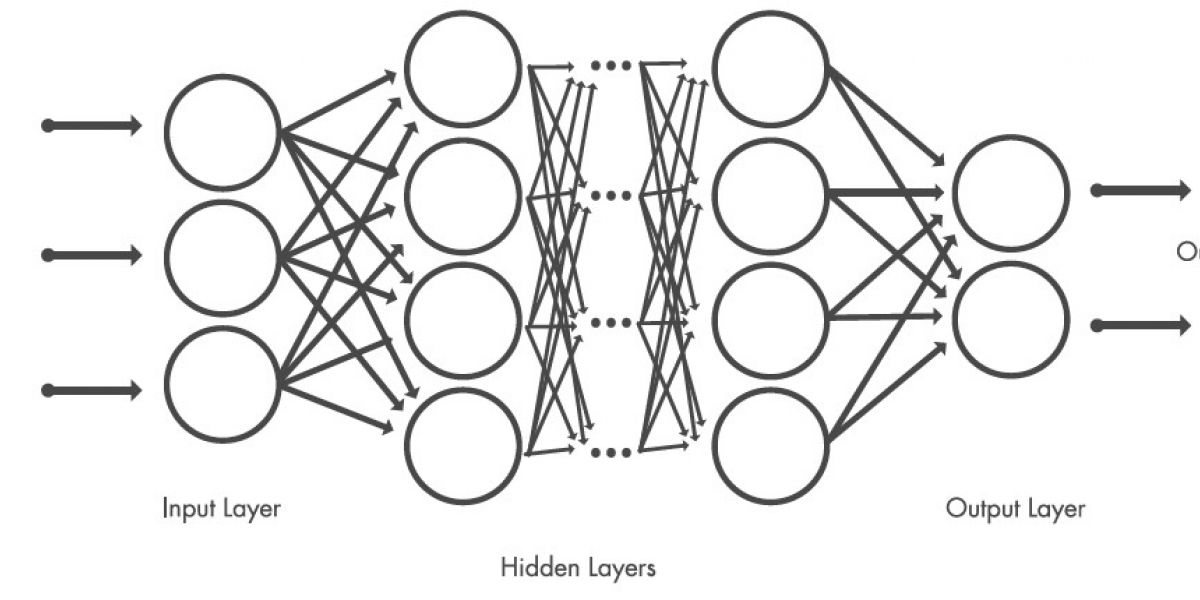
\includegraphics[width=15cm]{Bilder/Deep-Learning.jpg}
		\caption{Hidden Layer}
		\label{Deep Learing von Technik-und-Wissen}
	\end{center}
\end{figure}
% https://www.technik-und-wissen.ch/assets/images/4/1-Mathworks-Deep-Learning-80166094.jpg
\\Ein künstliches neuronales Netz wird mit dem Zweck aufgebaut, eine bestimmte Aufgabe zu lösen. Extra dafür müssen Testdaten aufbereitet werden. Diese Art der Daten, beispielsweise Bilder, soll das fertig trainierte Netz richtig interpretieren können. Testdaten sind Daten, bei dem das korrekte Ergebnis zu jedem Test bekannt ist.
\\\\
Am Anfang ist das künstliche neuronale Netz meist mit relativ zufälligen Werten und Verbindungen vorbelegt. Testdaten werden dem zu trainierenden Netzwerk an die Eingangsschicht übergeben. Diese durchlaufen das Netz. Das Ergebnis wird an der Ausgabeschicht überprüft. Die Ausgabeschicht besteht im einfachsten Fall aus zwei Neuronen, beispielsweise 'Gesicht erkannt' oder 'kein Gesicht', an dem gemessen wird, wie viel gewichtete Signale ankommen. Diese summiert, ergeben die Endergebnisse der Berechnungen und das Neuron mit dem höchsten Gewicht, ergibt die Antwort.
\\\\
Neuronale Netze sind für Menschen ab einer gewissen Größe nicht mehr nachvollziehbar. Somit kann nur die Eingabe mit der Ausgabe verglichen werden, um auf die Korrektheit der Aufgabenlösung zu prüfen. Ziel ist es durch möglichst viele und umfangreiche Testdaten das Netzwerk so einzustellen, dass diese nicht nur die Testdaten richtig beantwortet, sondern auch unbekannt Daten korrekt interpretiert.
\\\\
Um eine Aufgabe, wie 'Gesicht in Bild erkennen', zu trainieren, wird nicht nur ein Netz mit Zufallswerten und Verbindungen generiert sondern tausende. Alle werden mit den gleichen Testdaten geprüft und für jedes Netz ein Mittelwert über die Korrektheit der Antworten erstellt. Da alle Netze Initial mit Zufallswerten belegt sind, haben die meisten Netze eine Erfolgsrate von ca. 50 Prozent. Die Netze mit den höchsten Erfolgsraten, mit beispielsweise mehr als 55 Prozent, werden behalten, der Rest wird verworfen. Die erfolgreichsten Netze werden mehrfach kopiert und bei jedem Kopiervorgang individuell leicht verändert und erneut getestet. Die Besten werden wieder genommen und leicht modifiziert kopiert und schlechteren verworfen. 
\\\\
Nach einer gewissen Anzahl an Iterationen entscheidet das Netz nicht mehr willkürlich, sondern scheint intelligent die Aufgabe zu lösen. Dieser Iterationsschritt kann unendlich oft laufen, jedoch empfiehl es sich, je nach Anwendungsfall, ab einer gewissen Erfolgsrate das Training zu beenden oder neue Testdaten zu verwenden. Als Ergebnis des Prozesses erhält man durch Deep Learning ein trainiertes künstliches neuronales Netz, das im Allgemeinen als KI bezeichnet wird.
\\\\
Die KI kann nun die Testdaten nahe zu perfekt interpretieren. Trotzdem muss nun noch weiter überprüft werden, ob die KI auch unbekannte Daten korrekt interpretiert. Fehlverhalten einer KI kann leicht übersehene werden, da es fast unmöglich ist, jeden Testfall abzudecken. Beispiele von KIs mit Fehlverhalten und wie sie genau entstehen, werden im nächsten Abschnitt genauer betrachtet.


\chapter{Problemstellung Fehlverhalten von künstlichen neuronalen Netzen}
\section{Was sind Fehlverhalten von künstlichen neuronalen Netzen?}
\label{section:KIBias}
Ca. 4 Jahre entwickelte Amazon einen Algorithmus, welcher unter mehreren Bewerbungstexten automatisch die besten Bewerber herausfiltern sollte. Dabei bezog die Software sich auf voran gegangene Bewerbungen, verdeutlichte dabei aber ein grundlegendes Problem des maschinellen Lernens in seiner aktuellen Form.\\\\
Der Algorithmus hatte mit den Datensätzen der angenommen Bewerber trainiert und lernte daraus welche Eigenschaften Amazon bevorzugt. Weil das Unternehmen aber Teil einer von Männern dominierten Industrie ist, waren in den zugrunde gelegten vergangenen zehn Jahren vor allem Männer eingestellt worden. Daraus resultierte, dass Frauen grundsätzlich schlechter bewertet wurden, selbst wenn gar kein Geschlecht angegeben wurde und dieses z.B. nur durch Frauenvereine erkennbar wurde. Die KI blieb diesen Auswahlkriterien treu und bevorzugte vorwiegend Männer.\cite{amazon} \\\\
Dieses Fehlverhalten der KI führte dazu, dass die Software nicht genutzt werden konnte, bzw. nach Anpassungen nur eine beratende Funktion besaß.
\\\\
Unbekannt ist dieses Verhalten allerdings nicht. Es gibt weitere Fälle in der eine KI so wirkt, als hätte sie Vorurteile gegenüber manchen Gruppen/Geschlechter/Religionen, welche allerdings Fehlverhalten sind und durch den Menschen antrainiert wurden.

\section{Garbage in - Garbage Out - Wie entstehen Fehlverhalten von künstlichen neuronalen Netzen?}
Wie in vorangegangen Beispielen bereits erwähnt wurde, wird Künstliche Intelligenz in vielen Bereichen eingesetzt. Die Hoffnung solcher Anwendungen, liegt eigentlich darin, Vorurteile zu vermeiden und Prozesse fairer zu gestalten, da eine Maschine grundsätzlich keinen Unterschied zwischen Schwarz und Weiß, Mann und Frau oder Jung und Alt erkennt.
\\\\
Anhand des Beispiels aus \ref{section:KIBias} sieht man, dass dies nicht der Fall ist, da die Daten, mit welchen die KI lernt, zentralen Einfluss auf das Ergebnis hat. Meist ist es nicht möglich Daten zu finden, welche nicht bereits Vorurteile, enthalten. Solch verzerrte Trainingsdaten, werden unter Bezug auf ihre Zusammensetzung, auch als WEIRD Samples(western, educated, industrialized, rich and democratic societies) bezeichnet.% \cite{BiasInKI} Weiß nicht ob ich das Zitieren will%
\\\\
Ein weiteres Problem ist die fehlende Diversität auf Seiten der/die Entwickler/innen. Nur 15\% bei Facebook und 10\% bei Google in der KI Entwicklung sind Frauen. Für dunkelhäutige Menschen ist es noch schlimmer. Bei Google z.B. sind nur 2,5\% und bei Facebook und Microsoft 4\% dunkelhäutige Mitarbeiter\cite{Discriminating}.
\\\\
Daher kommt der Ausdruck "Garbage in - Garbage Out", dass heißt benutzt man fehlerhafte Daten oder welche, die Vorurteile beinhalten, erhält man fehlerhafte oder mit Vorurteilen belastete Ergebnisse.

\section{Probleme durch Fehlverhalten von künstlichen neuronalen Netzen}
Durch die bereits genannten Beispielen in den vorherigen Kapiteln, werden Probleme deutlich. Das Fehlverhalten einer KI kann zu Diskriminierung einzelner Geschlechter/Gruppen oder Kulturen führen. Ein anderes Problem wird aber deutlich, wenn man ein Beispiel aus der Medizin anschaut.
\\\\
In der USA existiert eine KI, welche die Gesundheitsversorgung möglichst effektiv gestalten soll. Diese soll eine Person mit besonderem Pflegebedarf identifizieren. Eine im Oktober 2019 veröffentlichte Studie zeigt allerdings auf, dass Menschen mit Afroamerikanischen Wurzeln bei gleicher Krankheitsschwere, seltener für extra Pflege vorgeschlagen wurden als Weiße\cite{Gesundheitsversorgung}. \\
Dies führt dazu das Afroamerikaner eine niedrigere Gesundheitsversorgung haben als andere und dies kann zu großen Gesundheitliche Problemen führen.
\\\\
Ein weiteres Beispiel nannte das Heise Magazin 2017\cite{heise}. Das Online Magazin erwähnte die Software COMPAS, welche auch in der USA verwendet wird und dort in mehreren Bundesstaaten zum Einsatz kommt. COMPAS steht für „Correctional Offender Management Profiling for Alternative Sanctions“ und gibt vor, das Rückfallrisiko von Straftätern verlässlich berechnen zu können.
\\\\
COMPAS errechnet für jeden Delinquenten einen individuellen Risk Score, welcher auf das spätere Strafmaß Auswirkungen hat.
In die Risikobeurteilung des Algorithmus fließen eigene Vorstrafen, eventuelle Vorstrafen naher Verwandter, Alkohol- und Drogenmissbrauch, soziale Bindungen, usw..
\\\\
Falls der Risk Score eines Verurteilten nun zwischen 1 und 10 ist, lässt der Richter keine Bewährung mehr zu sondern schickt ihn präventiv hinter Gitter.
Das Problem hierbei ist, dass der Algorithmus nicht offen gelegt wird und somit wird dem Algorithmus blind vertraut, ohne überprüfen zu können, wie dieser Score zustande kam.
\\\\
Wie Heise Magazine weiter berichtete, belegte allerdings 2016 eine Studie der Investigativ-Plattform ProPublica, dass die COMPAS-Algorithmen beispielsweise schwarzen Angeklagten grundsätzlich ein höheres Risiko attestieren, erneut straffällig zu werden, als dies tatsächlich der Fall ist. Bei weißen Angeklagten ist es hingegen genau umgekehrt.
\\\\
Falls solche Algorithmen blind vertraut werden, kann dies zu gravierenden Folgen eines Verdächtigen führen, welcher zu unrecht ein ganzes Leben hinter Gitter sitzen könnte.

\chapter{Sicherheitsprobleme durch Fehlverhalten von künstlichen neuronalen Netzen}
Genauer auf die Probleme davon eingehen, auf Beispiele aus \ref{section:KIBias} eingehen und Probleme erläutern, die dadurch auftreten könnten? \\\\
Sicherheit definieren, differenzieren von englisch safety und security etc.

\chapter{Prävention der Fehlverhalten von künstlichen neuronalen Netzen}
\label{chapter:main}
\section{Erkennung von Fehlverhalten von künstlichen neuronalen Netzen}
Erkennung von Fehlverhalten von künstlichen neuronalen Netzen durch Menschen/Computer.
\section{Testdaten Aufbereitung}
Wie kann ich die Testdaten aufbereiten, damit kein Fehlverhalten von künstlichen neuronalen Netzen auftritt?

\chapter{Analyse}
Analyse auf Umsetzbarkeit der Lösungsansätze aus \ref{chapter:main}.

\chapter{Fazit}
Zusammenfassung und Ergebnis.



\backmatter
%%%%%%%%%%%%%%%%%%%
%% create tables list
%%%%%%%%%%%%%%%%%%%
\listoftables

%%%%%%%%%%%%%%%%%%%
%% create listings list
%%%%%%%%%%%%%%%%%%%
%\lstlistoflistings
%\addcontentsline{toc}{chapter}{Listings}

\cleardoublepage
\phantomsection
\addcontentsline{toc}{chapter}{Literatur}
\printbibliography

\end{document}
